% -*- root: ../main.tex -*-
%!TEX root = ../main.tex
% this file is called up by main.tex
% content in this file will be fed into the main document
% vim:textwidth=80 fo=cqt

The  equations   presented  in~\cref{sec:spmmodeldevelopment}   are  well-known,
self-sufficient and  fully descriptive so  as to implement the  basic \gls{spm}.
Although  numerical implementation  of  circuit-oriented cell  models have  been
considered~\cite{Plett2004,Plett2004a,Plett2004b,Plett2006}, there  has yet been
no treatment  of this critical  aspect in \gls{spm} modelling  literature. Since
this thesis has a strong focus  towards enabling the use of physics-based models
in an embedded environment, at least the numerical aspects of implementing these
equations needs  to be  discussed. The finer  details and  practical engineering
consideration of  real-time programming,  in particular  the integration  of the
cell model into the pack and its  interaction with other elements and aspects of
a typical vehicular  drivetrain controller is beyond the scope  of this academic
work. Nevertheless, the  discussion here aims to lower the  barrier to real-time
implementation and is a  unique contribution of this work in  the context of the
cell modelling art.

\subsection{Continuous-time Implementation}

\subsubsection*{Analytical solution}

Although not  explicitly given  in \gls{spm}  literature, from  \gls{lti} system
theory,  an   analytical  solution   for  the  continuous-time   state  equation
of~\cref{eq:LTIstatespace} is given by
\begin{align}
    \mathbf{x}(t) &= e^{A (t-t_0)}\mathbf{x}(t_0) + \int_{t_0}^{t}e^{A (t-τ)}B \mathbf{u}(τ)\,dτ \label{eq:genanalyticctssoln}
    \\
    \shortintertext{With a standard \gls{ivp}, $t_0 = 0$}
    \mathbf{x}(t) &= e^{A t}\mathbf{x}(0) + \underbrace{\int_{0}^{t}e^{A (t-τ)}B \mathbf{u}(τ)\,dτ}_{\text{convolution integral}}\label{eq:analyticalctssoln}
\end{align}

The matrix exponential $e^{At}$ is known as the state-transition matrix and is
defined as
\begin{equation}
    e^{A t} ≜ \mathcal{L}^{-1}\left\{(s I - A)^{-1}\right\}
\end{equation}
although several methods exist for its efficient numeric
computation~\cite{Moler2003}.

The  analytical  solution  of~\cref{eq:analyticalctssoln}   can  be  applied  to
obtain  the matrix-vector  state equation~\cref{eq:threestatesmatrixvec}  of the
\gls{spm}.  Once  the  state-solution  is   obtained  at  any  time-step,  after
evaluating  the  surface   concentrations  as  per~\cref{eq:csurfposfromcavgpos}
and~\cref{eq:csurfnegfromcavgneg} and  the resulting  values may  be substituted
into the  output equation of~\cref{eq:spmbasicoutputvoltagefinal} to  obtain the
cell terminal voltage.

\subsubsection*{Numerical considerations for continuous time implementation}

The procedure described  thus far has a practical limitation.  The input current
$I(t)$ to the cell is defined as a continuous quantity. Although for the purpose
of characterising  the cell's  behaviour, it is  possible to  use pre-determined
continuous-functions as  load profiles  (\eg{} sinusoidal waveforms  for virtual
\gls{eis} testing), it is desirable to  evaluate the model's response to typical
real-life  conditions. In  a vehicular  application,  only the  samples of  cell
current  measured by  sensors at  discrete-time  intervals are  reported to  the
\gls{bms}. A \gls{zoh}  operation is used at the model's  input, \ie{} the level
of current is  assumed to be held constant between  two successive measurements.
Current profiles can be computed from standard drive cycle data.

It     is    tedious     to     hand-compute     the    convolution     integral
of~\cref{eq:analyticalctssoln}.  However,   a  variety  of  state   of  the  art
adaptive-time  solvers  employing  numerical  schemes  such  as  Dormand-Prince,
Runge-Kutta,  Collocation  or  Backward  Difference Formulae  are  available  to
efficiently  handle  such \gls{ode}s.  Given  that  lithium concentrations  vary
smoothly over time  without abrupt discontinuities, a  standard non-stiff solver
of moderate order  shall suffice. A single line of code  using MATLAB's ode45
solver can implement the time integrator, \eg{} \\ \mintinline{matlab}{[~,x_new] =
ode45(@(t,x) stateEqn(x,Ik,spm_params), t_span, x_old); }

Since  the direction  of applied  current  is susceptible  to sudden  reversals,
(\eg{}  due to  acceleration and  braking events  for a  vehicular application),
the  solver   needs  to   be  stopped  and   re-started  every   sample  period.
\Cref{alg:ctstimespm} shows the  sequence of operations in  a desktop simulation
of the continuous time \gls{spm} on  a digital computer. The source code listing
of an example implementation in MATLAB is provided in~\cref{sc:ctstimespm}.

% -*- root: ../main.tex -*-
%!TEX root = ../main.tex
% this file is called up by main.tex
% content in this file will be fed into the main document
% vim:nospell

\begin{algorithm}[!htbp]
    \caption{Continuous time \protect{\gls{spm}}}\label{alg:ctstimespm}
    \begin{algorithmic}[1]
        \Require Load profile \Comment{\eg{} a \texttt{csv} file of $t$ vs. C-rate}
        \Require \gls{spm} parameter set  \Comment{\eg{} stored in a struct \texttt{params}}
        \Userdata $z[1], t_\text{f,user}$, $t_\text{f,condition}$, cell capacity $I_\text{1C}$, sample rate $T_s$ \Comment{$t_\text{f,condition} \in  \left\{\texttt{max}, \texttt{min}\right\}$}
        \Ensure  $z[1], V_\text{cell}[1]$ within limits \Comment{index $[k=1] \wedgeq \text{time } (t=0) $}
        \Procedure{Simulate\gls{spm}}{}%{$z[1],t_\text{f,desired},T_s,I_\text{1C},\texttt{params}$}
            \State {$t_\text{f,desired} =
                \begin{cases}
                   \max(t_\text{f,user},t_\text{f,profile}),
                        &\text{%\scriptsize
                    if $t_\text{f,condition}$ == \texttt{max};}\\
                    \min(t_\text{f,user},t_\text{f,profile}),
                    &\text{%\scriptsize
                otherwise.}
                \end{cases}$} \Comment{\parbox[t]{0.25\textwidth}{may terminate early due to cut-off violations}}
                    \FullComment{\scriptsize Flexible end time. Extrapolate last C-rate from profile until $t_\text{f,desired}$ if necessary.}
            \State $N_\text{max} \gets \ceil*{\frac{t_\text{f,desired}}{Ts}} + 1$ \Comment{max iterations assuming no cut-offs}
            \State Allocate storage of size $\mathbb{R}^{N_\text{max}\times 1}$ for each simulation variable
            \State Compute $\mean{c}_\sneg$[1] as per~\cref{eq:csfluxinitialcondition}
            \State $I[1] \gets I_\text{1C} \times  \text{C-rate}[1], \quad \mathbf{x}[1] \gets \vect{0,0, \mean{c}_\sneg[1]}$ \Comment{ $\text{C-rate}[1]$ from profile}
            \State $V_\text{cell}[1] \gets \textsc{ComputeCellVoltage}(\textbf{x}[1],I[1],\texttt{params})$ \Comment{from direct feedthrough}
            \For{$k \gets 2 : N_\text{max}$}
                \State $I[k] \gets $ interpolate from profile using \gls{zoh}
                \State Solve continuous-time equation~\cref{eq:threestatesmatrixvec} \Comment{solver IC set to $x[k-1]$}
                \State $\mathbf{x}[k] \gets $ last time-entry  vector of soln.\  matrix \Comment{from an adaptive solver \eg{} MATLAB's \texttt{ode45}}
                \State Compute $z[k]$ as per~\cref{eq:soccomputation}
                \State $V_\text{cell} \gets \textsc{ComputeCellVoltage}(\textbf{x}[k],I[k],\texttt{param}) $
                \If {$z[k] \text{ or } V_\text{cell}[k]$ exceeded cut-off limits}
                    \State $k \gets k - 1$ \Comment{data from last  step is invalid}
                    \State \textit{break};
                \EndIf
            \EndFor
        \EndProcedure

        \OutputEqn{\textbf{x},I,\texttt{params}}
            \State Compute $c_\snegsurf$ as per~\cref{eq:csurfnegfromcavgneg}
            \Comment{consider saturating \ie{} $c_\snegmin \le c_\snegsurf \le
            c_\snegmax$}
            \State Compute $\mean{c}_\spos$ as per~\cref{eq:csposbulkfromcsnegbulk}
            \State Compute $c_\spossurf$ as per~\cref{eq:csurfposfromcavgpos}
            \State Compute $V_\text{cell}$ as per~\cref{eq:spmbasicoutputvoltagefinal}
        \EndOutputEqn%
    \end{algorithmic}
\end{algorithm}


The continuous time \gls{spm} algorithm has limited practical use. Computing the
convolution integral or deploying \gls{ode}  solver code in a microcontroller is
challenging  and introduces  a  substantial computational  burden. Although  the
continuous time  model can  be used for  desktop simulation,  more sophisticated
physics-based  models  are available  for  this  task. However,  the  continuous
time  \gls{spm} has  an  important application,  \viz{}  estimation of  physical
parameters  which will  explored  in~\cref{sec:spmparameterestim}. However,  for
online  deployment  for state  estimation  and  control tasks,  a  discrete-time
version of the model suitable for real-time implementation is needed.

\subsection{Conceptual Overview of Real-Time Processing}

The equations  in~\cref{sec:spmmodeldevelopment} are derived  in continuous-time
form. In particular, the  state equation given by~\cref{eq:threestatesmatrixvec}
describes  the  continuous   time  dynamic  evolution  of   quantities  such  as
the  bulk  concentration   and  mean  radial  flux  rate.   However,  a  typical
embedded  controller  such  as  that  used in  a  vehicular  \gls{bms}  operates
in   discrete-time~\cite{Andrea2010}.  This   implies  that   \emph{samples}  of
voltage,  current and  temperature measurements  are obtained  at a  period time
interval~$T_s$. The computations of the model equations and updating of solution
variables  (such as  bulk  concentrations and  terminal  voltage) are  performed
between two successive data acquisition events from the sensors.


Control-oriented  physics-based cell  models  such as  the  \gls{spm} and  their
associated  computations can  be  considered  as a  modular  subsystem within  a
\gls{bms}. A  single \gls{bms} often  provides a  whole host of  other auxiliary
functionality such as cell  balancing, protection, diagnostics and data-logging.
Although  thermal   management  tasks  are  typically   delegated  to  dedicated
controllers,  the  \gls{bms} software  routines  handle  data exchanged  between
various  controllers on  the vehicular  communication bus.  While some  of these
tasks such  as book-keeping and  diagnostics can be done  at a low  rate, others
such as  those involving measurements  from cell and  model-related computations
need to be performed with high priority.

\begin{figure}[tbh]
    \savebox{\algboxA}{%
        \begin{varwidth}[b]{0.65\linewidth}
            \begin{flushleft}
                \begin{algorithmic}[0]

                    \Initialise \gls{soc} \& other global variables
                    \Ensure voltage, current \& temperature limits
                    \Procedure{Main}{$ $}

                    \State configure interrupts
                    \State enable timers
                    \State $\vdots$
                    \While{\textproc{True}} \Comment[\scriptsize]{until ``key off" or shutdown}
                    \State background task \#1 \Comment[\scriptsize]{diagnostics/protection}
                    \State background task \#2 \Comment[\scriptsize]{\textproc{canbus} communication}
                    \State $\vdots$
                    \If{\texttt{needs\textunderscore balancing == 1}}
                    \Function{PackBalance}{$n_\text{cells}$,$\text{\gls{soc}}_i$,$v_i$}
                    \State \textit{subroutine for pack balancing}
                    \State $\vdots$
                    \EndFunction
                    \EndIf
                    \State $\vdots$
                    \State background task \#$n$ \Comment[\scriptsize]{supervisory reporting}
                    \EndWhile
                    \EndProcedure
                \end{algorithmic}
            \end{flushleft}%
        \end{varwidth}%
    }%
    \savebox{\algboxB}{%
        \begin{varwidth}[b]{0.65\linewidth}
            \begin{flushright}
            \begin{algorithmic}[0]
                \ISR[]{}
                \State read new sensor data from ADC
                \Function{ComputeSPM}{$i_{k-1}$, params}
                \State evaluate spm model equations
                \State $\vdots$
                \State compute model output voltage
                \Function{SOCEstimator}{$v_\text{model}$,$v_\text{meas}$}
                \State \textit{state estimation subroutine}
                \State $\vdots$
                \EndFunction
                \Function{ICEControl}{$ $}
                \State $\vdots$
                \State write control outputs to DACs
                \EndFunction
                \EndFunction
                \END
            \end{algorithmic}
            \end{flushright}
        \end{varwidth}%
    }
    \centering
    \framebox[\textwidth]{
      \subcaptionbox{background processes (low priority)\label{subfig:bgRTprocess}}{\usebox{\algboxA}}
        % \quad
        \hfill
        \subcaptionbox{foreground processes (high priority)\label{subfig:fgRTprocess}}{%
            \raisebox{\dimexpr.5\ht\algboxA-.5\ht\algboxB}{%
                \usebox{\algboxB}%
            }%
        }%
    }
    \caption[Overview of real-time software implementation of a typical
    \gls{bms}]{Overview of the real-time software implementation of a typical
        \gls{bms}. Through an interrupt-driven architecture for time-critical tasks as
        as state estimation and control, the same processor can be
        efficiently utilised by employing its idle CPU cycles for background
        tasks such as diagnostics, fault logging and book-keeping.}
    \label{fig:basicRTCsoftwarearch}
\end{figure}

\Cref{fig:basicRTCsoftwarearch}  shows  an  example   of  a  \gls{bms}  software
implementation in an embeddded microcontroller. The vast array of functionality
performed by the \gls{bms} can be grouped and managed as two separate processes --
\begin{enumerate*}[label=\itshape\alph*\upshape)]
    \item Background thread and
    \item Foreground thread.
\end{enumerate*}
The   background   thread  runs   continuously   within   the  main   loop   and
processes instructions sequentially.  \Cref{subfig:bgRTprocess} shows an example
illustration  of  typical  background  tasks   that  a  \gls{bms}  handles.  The
high-priority tasks  are triggered by  an interrupt and the  supervisory control
loop suspends  the presently executing  background task for later  resumption. A
typical  example of  such  an  interrupt driven  process  is  the evaluation  of
the  \gls{spm} model  equations  and  computation of  control  outputs as  shown
in~\cref{subfig:fgRTprocess} and is discussed further.

\begin{figure}[htb]
    \centering
    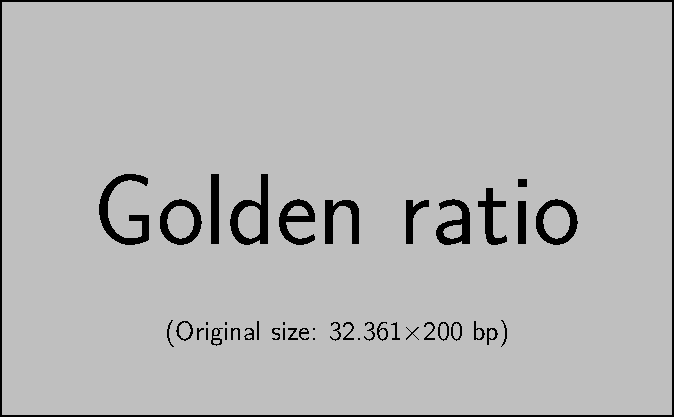
\includegraphics[width=\textwidth]{placeholder_images/example-image-golden.pdf}
    \caption[Timing diagram of a real-time software loop of a \gls{bms}]
    {Timing diagram of a real-time software loop of a \gls{bms}. The sequence of events within one sample period $T_s$ in relation
        to the base clock of the controller is shown. Particular emphasis is
        placed on depicting the handling of \gls{isr} requests pertinent to cell
        models. Other background tasks performed by the CPU is de-emphasised.
        Moreover, the integration
        of the  \gls{bms} software loop within  the larger  scope of  a master  vehicular
    controller is not shown.}
    \label{fig:timingdiagramBig}
\end{figure}

\Cref{fig:timingdiagramBig} depicts  an exploded view  of the timing  aspects of
the \textsc{Interrupt  Service Routine}  presented in~\cref{subfig:fgRTprocess}.
Upon   the  expiry   of  an   on-chip  timer   calibrated  against   a  baseline
precision-clock,  hardware  interrupts are  raised  by  one or  more  \gls{adc}s
associated with voltage/current sensors mounted on cells. The \gls{isr} disables
the  interrupt  and  reads  the  samples   of  data  from  the  \gls{adc}s  into
software. At  the end of this  process, the \gls{isr} rearms  the interrupts and
simultaneously sends and acknowledgement to the appropriate sensor which reloads
its timer.  The \gls{spm}  model equations  are then  evaluated in  software and
resulting computational variables such as  voltage and concentrations is used in
other activities such as state estimator. If the \gls{bms} also performs control
tasks, \eg{} regulating  the coolant-flow rate or  \gls{ice} state-toggling such
as  in the  hysteresis control  of a  series hybrid,  these control  outputs are
written to the relevant \gls{dac}s.

\subsection{Sample Delay Considerations}

\begin{figure}[h]
    \centering
    \hrulefill
    \caption[Timeline of \gls{bms} activities over multiple CPU cycles of a real-time
    controller]{A timeline view of CPU activities within each sample time
        depicting the repeating blocks of the execution sequence is shown over a
        larger horizon. The vast majority of the CPU cycle is spent in idling or
    background tasks. The servicing of \gls{isr} occupies a relatively small fraction.}
    \label{fig:timingdiagramSmall}
\end{figure}

\Cref{fig:timingdiagramSmall} shows a timeline view of all CPU activities across
a larger  time horizon.  The CPU's  load factor is  the ratio  of time  spent in
foreground requests to  its idling time. While a high  load factor is beneficial
in  terms of  efficient  usage  of resources,  it  adversely  affects the  power
efficiency of the chip.

For  Li-ion  cell  modelling,  a  sampling interval  of  $T_s  =  1$\si{\second}
is   commonly  used,   thus  aiming   to   capture  the   cell  dynamics   below
\SI{1}{\hertz}\footnote{In  the ideal  case, according  to the  Nyquist sampling
theorem. However, in practice the frequency  range is lower.}. The CPUs clock is
several \si{\MHz}, a vast  majority of which is spent in  background tasks or in
sleep mode. Furthermore,  a low-latency \gls{isr} code is employed  in the tasks
of reading the  \gls{adc} value, evaluating the model equations  and writing any
control outputs to  the \gls{dac}. Using a simplified  physics-based models such
as the \gls{spm} helps in achieving a low-latency throughput for the \gls{isr}.

The overall implication of such a scheme  is that any \emph{delays} owing to the
sample and  hold process  at the model  input and outputs  can be  neglected. In
conventional sampled-data systems, control delays may be analysed by considering
a multiplicative factor of $e^{-sλ}$ in the Laplace domain transfer function of
the system.  Delay parameters of  $λ = 0.5  T_s$ or $λ  = 1 T_s$  are commonly
employed as  conservative estimates. However,  owing to the extremely  small CPU
load factor considered as established here, this delay factor is omitted in this
thesis for discrete-time formulation of the \gls{spm} model.


\subsection{Discrete-Time \Gls{spm} formulation}

\begin{figure}[htb]
    \centering
    % show block diagram cross-referencing equation and a question mark for the
    % dt system
    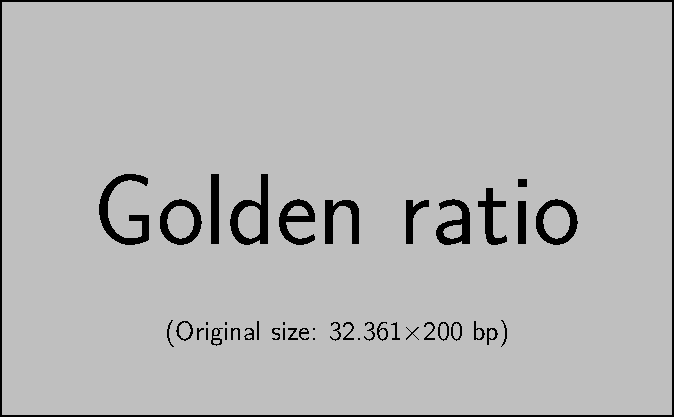
\includegraphics[width=0.75\textwidth]{placeholder_images/example-image-golden.pdf}
    \caption[Block-diagram of continuous and discrete-time systems]{Block-diagram of the plant model and associated signals of a continuous-time system and its discrete-time counterpart}
    \label{fig:blockdiagctsdisc}
\end{figure}

\Cref{fig:blockdiagctsdisc} shows  a block  diagram representation of  the plant
model its associated input and output signals. Due to the sampling and \gls{zoh}
operation  at  the  \gls{adc}  input  to  the  system,  the  input  signals  are
transformed  from  being  simple  continuous time  quantities  to  discrete-time
sequences,  \ie{} $u(t)  \mapsto  u[k]$  and $y(t)  \mapsto  y[k]$,  where $k  =
0,1,\dots,∞$ is the sample index  corresponding to the continuous time instant
$t_k  = kT_s$.  The continuous  time plant  model represented  by the  \gls{ode}
system of~\cref{eq:threestatesmatrixvec} is replaced  by a discrete-time process
and modelled by a \emph{difference} equation which is to be determined.

Consider       the       general      continuous-time       solution       given
by~\cref{eq:genanalyticctssoln}. Let $t_0 = k T_s$ and $t = (k+1)T_s$, where $k  =
0,1,\dots,∞$. Therefore,
\begin{alignat}{2}
    x(t_0) & = x(kT_s)     & & \equiv x[k] \\
    x(t)   & = x((k+1)T_s) & & \equiv x[k+1]
\end{alignat}
Substituting these relationships into~\cref{eq:genanalyticctssoln},
\begin{equation}
    \mathbf{x}[k+1] = e^{A T_s}\mathbf{x}[k] + \int_{k T_s}^{(k+1)T_s}e^{A ((k+1)T_s-τ)}B \mathbf{u}(τ)\,dτ \label{eq:intermediatediscrete}
\end{equation}
With the  \gls{zoh} scheme  discussed here, $u(\tau)$  remains constant  from $k
T_s$ to $(k+1)T_s$,  and is equal to $u(kT_s)$, \ie{}  $u[k]$. Consider a change
of variable definition  for the dummy variable of integration  $\tau$ as $\eta =
(k+1)T_s -  \tau$. Thus,  $\tau = (k+1)T_s  - \eta$. Hence,  $d \tau  = -d\eta$.
Substituting these into~\cref{eq:intermediatediscrete},
\begin{align}
    \mathbf{x}[k+1] &= e^{A T_s}\mathbf{x}[k] + \left[\int_{T_s}^{0}e^{A \eta }B \right] u[k]\,{-d\eta}\\
    \shortintertext{Reversing the order of integration leads to}
    \mathbf{x}[k+1] &= e^{A T_s}\mathbf{x}[k] + \left[\int_{0}^{T_s}e^{A \eta }B \,{d\eta} \right] u[k] \label{eq:disctimefulleqn}
\end{align}

\Cref{eq:disctimefulleqn} represents a discrete-time state-space representation
of the dynamics of the system whose generic representation is given by the
difference equation
\begin{equation}\label{eq:discgenericLTI}
    \mathbf{x}[k+1] = A_d x[k] + B_d u[k]
\end{equation}
where $A_d = e^{A T_s}$ and $B_d = \int_{0}^{T_s}e^{A \eta}B
\,{d\eta}$.
If the continuous-time system matrix, $A$ is invertible, a closed form
expression for $B_d$ is obtained as
\begin{align}
    B_d &= A^{-1}(A_d - I_n)B && \text{(if $A^{-1}$ exists)}
\end{align}
For the continuous time system matrix $A$ of the \gls{spm}, its determinant is
zero, \ie{}
\begin{equation}
\begin{vsmallmatrix}
    -30\frac{D_\spos}{R_\ppos^2} & 0                            & 0 \\
    0                            & -30\frac{D_\sneg}{R_\pneg^2} & 0 \\
    0                            & 0                            & 0
\end{vsmallmatrix} = 0
\end{equation}
and hence  is not invertible.  This necessitates  an explicit evaluation  of the
integral in~\cref{eq:disctimefulleqn} for computation of the discrete-time input
matrix, $B_d$.

Since the only non-zero entries of the matrix lie along its main diagonal, \ie{}
its modes  are decoupled, the  matrix exponential  reduces to a  diagonal matrix
whose elements are simply the scalar exponentials of the original entries.
\begin{equation}\label{eq:A_dinit}
    A_d = e^{A T_s} = \exp\left(
\begin{bmatrix}
    -30\frac{D_\spos}{R_\ppos^2} & 0                            & 0 \\
    0                            & -30\frac{D_\sneg}{R_\pneg^2} & 0 \\
    0                            & 0                            & 0
\end{bmatrix} T_s \right)
\end{equation}
\begin{equation}\label{eq:A_d}
A_d =
\begin{bmatrix}
    e^{-30\frac{D_\spos}{R_\ppos^2} T_s} & 0                                    & 0 \\
    0                                    & e^{-30\frac{D_\sneg}{R_\pneg^2} T_s} & 0 \\
    0                                    & 0                                    & 1
\end{bmatrix}
\end{equation}
\begin{equation}\label{eq:B_dinit}
    B_d = \int_{0}^{T_s}e^{A \eta}B \,{d\eta}
\end{equation}
\begin{equation}\label{eq:B_dintermediate}
    B_d =\bigint_{0}^{T_s} \left( \begin{bmatrix}
            e^{-30\frac{D_\spos}{R_\ppos^2} \eta} & 0                                    & 0 \\
            0                                    & e^{-30\frac{D_\sneg}{R_\pneg^2} \eta} & 0 \\
            0                                    & 0                                    & 1
        \end{bmatrix}\cdot
        \begin{bmatrix}
            \frac{45}{2} \frac{\hphantom{-}1}{R_\ppos^2 A \, l_\text{pos} a_\spos F} \\
            \frac{45}{2} \frac{-1}{R_\pneg^2 A \, l_\text{neg} a_\sneg F} \\
            \hphantom{\frac{45}{2}} \frac{-3}{R_\pneg  A \, l_\text{neg} a_\sneg F}
    \end{bmatrix} \right) \, d\eta
\end{equation}
\begin{equation}\label{eq:B_d}
    B_d = \begin{bmatrix}
        \hphantom{-}\frac{3}{4} \frac{1 - \exp\left(-30\frac{D_\spos}{R_\ppos^2}\right)T_s}{D_\spos A \, l_\text{pos} a_\spos F} \\[1em]
        -\frac{3}{4} \frac{1 -
        \exp\left(-30\frac{D_\sneg}{R_\pneg^2}\right)T_s}{D_\sneg A \, l_\text{neg} a_\sneg F} \\[1em]
        \hphantom{-}\hphantom{\frac{3}{4}} \frac{-3 T_s}{R_\pneg  A \, l_\text{neg} a_\sneg F}
    \end{bmatrix}
\end{equation}

The    discrete-time    matrix-vector    system    presented    in~\cref{eq:A_d}
and~\cref{eq:B_d} have not  been presented in existing literature,  but is vital
to understanding  the implementation  of the  \gls{spm} in  digital controllers.
Although, simpler  alternatives such as  Forward Euler methods are  available to
approximate the time-derivative  of the state vector, they  suffer from problems
such as increasing  rate of local truncation error  per time-step, necessitating
the use of  very high sample rates,  which increases the burden  on the embedded
controller. The matrix exponential approach is superior in terms of accuracy and
stability across a wide range of sample rates.

For a pre-determined sample-rate, the matrix exponential and hence the $A_d$ and
$B_d$  matrices  can be  computed  offline  on a  desktop  and  stored into  the
non-volatile storage  of the embedded  controller to  be loaded onto  RAM during
operation. The vectorised implementation of the state dynamics presented here is
highly  efficient  and  directly  amenable for  use  in  classical  state-vector
algorithms. For the cell's terminal voltage computation, the basic structure and
form  of the  output  equation given  by~\cref{eq:spmoutputeqn} remains  intact,
except  that the  continuous time  variables $\left(\mathbf{x}(t),  u(t)\right)$
need to  be replaced  by their discrete-time  counterparts in  the corresponding
equation set~\crefrange{eq:spmbasicoutputvoltagefinal}{eq:csurfnegfromcavgneg}.
The discrete-time output function $h_d$ is evaluated  \emph{after}  updating  the state  vector  through~\cref{eq:discgenericLTI}.
\begin{equation}\label{eq:discspmoutputeqn}
    y[k+1] = h_d(\mathbf{x}[k+1],u[k+1])
\end{equation}

The complete  sequence of steps  to implement  the discrete-time variant  of the
\gls{spm}  is given  in~\cref{alg:disctimespm}. In  particular, it  can be  seen
that  the discrete-time  system  and  input matrices,  $A_d$  and  $B_d$ can  be
pre-computed  from the  parameter set  (refer to  line~\ref{algLine:computeAdBd}
in~\cref{alg:disctimespm}), using  the matrix  exponential approach.  In MATLAB,
this  can be  achieved by  passing the  arguments of  the matrix  exponential to
the  \verb+expm+ command.  The  vectorised implementation  of the  discrete-time
state equation  given in  line~\ref{algLine:discstateEq} is  a set  of efficient
linear  algebra  operations  consisting  of  simple  matrix-vector  product  and
vector-addition routines.

% -*- root: ../main.tex -*-
%!TEX root = ../main.tex
% this file is called up by main.tex
% content in this file will be fed into the main document
% vim:nospell

\begin{algorithm}[!htbp]
    \caption{Discrete time \gls{spm}}\label{alg:disctimespm}
    \begin{algorithmic}[1]
        \Require Load profile \Comment{\eg{} a \texttt{csv} file of $t$ vs. C-rate}
        \Require \gls{spm} parameter set  \Comment{\eg{} stored in a struct \texttt{params}}
        \Userdata $z[1], t_\text{f,user}$, $t_\text{f,condition}$, cell capacity $I_\text{1C}$, sample rate $T_s$ \Comment{$t_\text{f,condition} \in  \left\{\texttt{max}, \texttt{min}\right\}$}
        \Ensure  $z[1], V_\text{cell}[1]$ within limits \Comment{index $[k=1] \wedgeq \text{time } (t=0) $}
        \Procedure{Simulate\gls{spm}}{}%{$z[1],t_\text{f,desired},T_s,I_\text{1C},\texttt{params}$}
            \State {$t_\text{f,desired} =
                \begin{cases}
                   \max(t_\text{f,user},t_\text{f,profile}),
                        &\text{%\scriptsize
                    if $t_\text{f,condition}$ == \texttt{max};}\\
                    \min(t_\text{f,user},t_\text{f,profile}),
                    &\text{%\scriptsize
                otherwise.}
                \end{cases}$} \Comment{\parbox[t]{0.25\textwidth}{may terminate early due to cut-off violations}}
                    \FullComment{\scriptsize Flexible end time. Extrapolate last C-rate from profile until $t_\text{f,desired}$ if necessary.}
            \State $N_\text{max} \gets \ceil*{\frac{t_\text{f,desired}}{Ts}} + 1$ \Comment{max iterations assuming no cut-offs}
            \State Allocate storage of size $\mathbb{R}^{N_\text{max}\times 1}$ for each simulation variable
            \State Compute $\mean{c}_\sneg$[1] as per~\cref{eq:csfluxinitialcondition}
            \State $I[1] \gets I_\text{1C} \times  \text{C-rate}[1], \quad \mathbf{x}[1] \gets \vect{0,0, \mean{c}_\sneg[1]}$ \Comment{ $\text{C-rate}[1]$ from profile}
            \State \algemph{Compute $A_d$ and $B_d$ \Comment{as per~\cref{eq:A_d} and~\cref{eq:B_d}}}\label{algLine:computeAdBd}
            \State $V_\text{cell}[1] \gets \textsc{ComputeCellVoltage}(\textbf{x}[1],I[1],\texttt{params})$ \Comment{from direct feedthrough}
            \For{$k \gets 2 : N_\text{max}$}
                \State $I[k] \gets $ interpolate from profile using \gls{zoh}
                \State \algemph{$x[k] \gets A_d x[k-1] + B_d u[k-1]$ \Comment{\cref{eq:discgenericLTI}}}\label{algLine:discstateEq}
                \State Compute $z[k]$ as per~\cref{eq:soccomputation}
                \State $V_\text{cell} \gets \textsc{ComputeCellVoltage}(\textbf{x}[k],I[k],\texttt{param}) $
                \If {$z[k] \text{ or } V_\text{cell}[k]$ exceeded cut-off limits}
                    \State $k \gets k - 1$ \Comment{data from last  step is invalid}
                    \State \textit{break};
                \EndIf
            \EndFor
        \EndProcedure

        \OutputEqn{\textbf{x},I,\texttt{params}} \Comment{uses discrete-time variants of eqs, \ie{} at index $k$}
            \State Compute $c_\snegsurf$ as per~\cref{eq:csurfnegfromcavgneg}
            \Comment{consider saturating \ie{} $c_\snegmin \le c_\snegsurf \le
            c_\snegmax$}
            \State Compute $\mean{c}_\spos$ as per~\cref{eq:csposbulkfromcsnegbulk}
            \State Compute $c_\spossurf$ as per~\cref{eq:csurfposfromcavgpos}
            \State Compute $V_\text{cell}$ as per~\cref{eq:spmbasicoutputvoltagefinal}
        \EndOutputEqn%
    \end{algorithmic}
\end{algorithm}


Since   a    subsection   of   researchers   in    electrochemical   engineering
might   not  be   familiar  with   the   nuances  of   matrix  exponential   and
discrete-time  matrix  computations   (refer  to  line~\ref{algLine:computeAdBd}
in~\cref{alg:disctimespm}),   a   snippet   of  MATLAB   code   clarifying   the
computation  of  the   discrete-time  system  and  input   matrices,  $A_d$  and
$B_d$  is  given  in~\cref{codesnippet:computeAdBd}.  A  full  code  listing  of
an  example  discrete-time  \gls{spm}   implementation  in  MATLAB  is  provided
in~\cref{sc:disctimespm}.

\begin{listing}
\begin{minted}[mathescape,autogobble,bgcolor=mintedbg,escapeinside=||,texcomments=true]{matlab}
% Returns $A_d$ and $B_d$ matrices
A_cts = [-30*Ds_pos/(R_pos^2),                    0, 0; ...
                            0, -30*Ds_neg/(R_neg^2), 0; ...
                            0,                    0, 0];
% $A_d = e^{A T_s}$ \fontfamily{libertinus}\selectfont(see eqs.~\crefrange{eq:A_dinit}{eq:A_d})
A_disc = expm(A_cts*Ts); % $\mathtt{expm}$ command computes the matrix exponential

B_cts = [ (45/2)/(R_pos^2*a_pos*L_pos*F*A); ...
         (-45/2)/(R_neg^2*a_neg*L_neg*F*A); ...
             (-3/(R_neg*a_neg*L_neg*F*A))];

% $B_d = \int_{0}^{T_s}e^{A \eta}B \,{d\eta}$ \fontfamily{libertinus}\selectfont(see eqs.~\crefrange{eq:B_dinit}{eq:B_d})
B_disc = nan(size(B_cts));
B_disc(1) = B_cts(1)*(exp(A_cts(1,1)*Ts)-1)/A_cts(1,1);
B_disc(2) = B_cts(2)*(exp(A_cts(2,2)*Ts)-1)/A_cts(2,2);
B_disc(3) = B_cts(3)*Ts;
\end{minted}
\caption{Computation of discrete-time matrices $A_d$ and $B_d$ in MATLAB}
\label{codesnippet:computeAdBd}
\end{listing}

Thus,  a discrete-time  model  of  the basic  ~\gls{spm}  is  now available  for
implementation in an embedded gls{bms}. Further analysis of discrete-time issues
such  as  aliasing, quantisation  noise,  signal  pre-conditioning and  discrete
fourier analysis lies in the specialised engineering domain of signal processing
and falls outside  the scope of the  thesis. The results of  the basic \gls{spm}
are presented next in~\cref{sec:basicspmsimresults}.

\FloatBarrier

% % https://tex.stackexchange.com/questions/113719/cleveref-fails-to-reference-algorithms

% % https://tex.stackexchange.com/questions/110412/numbering-in-algorithmicx
% % https://tex.stackexchange.com/questions/65993/algorithm-numbering

% % https://tex.stackexchange.com/questions/203713/how-can-i-typeset-function-names-as-they-appear-in-algorithmic-environments
% % https://tex.stackexchange.com/questions/100346/typesetting-listofalgorithms-like-listoffigures-and-listoftables-using-titletoc
% % https://tex.stackexchange.com/questions/30363/how-do-i-define-a-new-command-in-algorithmicx

% % https://tex.stackexchange.com/questions/67908/customizing-the-algorithmic-package-break-and-loop-labels

% % https://tex.stackexchange.com/questions/69449/avoid-putting-statements-on-the-same-line-with-algorithmicx

% % \usepackage{float}
% % \newfloat{algorithm}{t}{lop}
% % Add \floatname{algorithm}{Algorithm} to capitalise the float name
